% Created 2013-01-21 Mon 17:10
\documentclass[11pt]{article}
\usepackage[utf8]{inputenc}
\usepackage[T1]{fontenc}
\usepackage{graphicx}
\usepackage{longtable}
\usepackage{float}
\usepackage{wrapfig}
\usepackage{soul}
\usepackage{amssymb}
\usepackage{hyperref}
\usepackage[margin=0.5in]{geometry}
\usepackage{listings}
\usepackage{mempatch}
\usepackage{color}
\lstset{frame=shadowbox, rulesepcolor=\color{blue}}
\definecolor{bluekeywords}{rgb}{0.13,0.13,1}
\definecolor{greencomments}{rgb}{0,0.5,0}
\definecolor{redstrings}{rgb}{0.9,0,0}
\definecolor{bgcol}{rgb}{0.98,0.98,0.98}
\lstdefinelanguage{D} {morekeywords={abstract,alias,align,asm,assert,auto,body,bool,break,byte,case,cast,catch,cdouble,cent,cfloat,char,class,const,continue,creal,dchar,debug,default,delegate,delete,deprecated,do,double,else,enum,export,extern,false,final,finally,float,for,foreach,foreach_reverse,function,goto,idouble,if,ifloat,immutable,import,in,inout,int,interface,invariant,ireal,is,lazy,long,macro,mixin,module,new,nothrow,null,out,override,package,pragma,private,protected,public,pure,real,ref,return,scope,shared,short,static,struct,super,switch,synchronized,template,this,throw,true,try,typedef,typeid,typeof,ubyte,ucent,uint,ulong,union,unittest,ushort,version,void,volatile,wchar,while,with,__FILE__,__LINE__,__gshared,__thread,__traits}, sensitive=false,morecomment=[l]{//},morecomment=[s]{/*}{*/},morestring=[b]", morestring=[d]', alsoletter={.}}
\lstset{morekeywords={class,private,public,protected,import,assert},basicstyle=\footnotesize\ttfamily,showspaces=false,showtabs=false,,breaklines=true,showstringspaces=false,breakatwhitespace=true,commentstyle=\color{greencomments},keywordstyle=\color{bluekeywords},stringstyle=\color{redstrings},backgroundcolor=\color{bgcol}}

\title{Code Generation}
\author{Daniel B Davidson}
\date{}

\begin{document}

\maketitle



\section{Purpose}
\label{sec-1}

  
  The purpose of this tech note is to outline a specific set of
  utilities for generating code. A general framework is described as
  well as specific support for \texttt{C++} and D.

\section{Template Approach}
\label{sec-2}


  The original code generation was done in Python using \emph{Cheetah}
  template engine. After a fresh look I decided to port to Ruby and
  the \emph{Tenjin} template engine. The differences between Python and
  Ruby are not great. One nice advantage of Ruby over Python is the
  much more natural support for \emph{string interpolation} which occurs
  quite often in code generation. An advantage of \emph{Tenjin} vs
  \emph{Cheetah} is that diagnostics/debugging is simpler. \emph{Tenjin} does a
  better job of taking you to the exact line of the template where
  there is a problem, when there is a problem.

\section{General Structure}
\label{sec-3}


  All code is generated from ruby scripts. The following is a
  description of the ruby supporting script files. All files listed
  below are relative to \texttt{codegen/ruby/lib}, which should be present in
  the \texttt{RUBYLIB} path. So, for example, to require the \texttt{id} module
  inside the \texttt{codegen} module you would require `codegen/id' which
  would be located at \texttt{codegen/ruby/lib/codegen/id.rb}

  

\begin{center}
\begin{tabular}{ll}
 module/file                &  purpose                                                                                   \\
\hline
 codegen/id                 &  Support for consistently dealing with \texttt{id's}, as in user variables. This           \\
                            &  was created after \texttt{C++} support, so used primarily in D code generation            \\
 codegen/cpp                &  Module with all cpp support classes                                                       \\
 codegen/cpp/tmpl           &  Folder with all \texttt{C++} \emph{Tenjin} templates                                      \\
 codegen/database/database  &  Module supporting code generation of \texttt{C++} Table Gateway Patter                    \\
 codegen/database/tmpl      &  Templates for generating \texttt{C++} database code                                       \\
 codegen/mongoid            &  Module supporting mongodb code generation                                                 \\
 codegen/mongoid/tmpl       &  Templates for generating \texttt{C++} code to access mongo database                       \\
 codegen/dlang              &  Module supporting generating D code                                                       \\
 codegen/dlang/tmpl         &  Templates for generating D code                                                           \\
 place.rb                   &  This file hides path names by providing named lookups of paths/files.                     \\
                            &  No hardcoding of non-relative paths should exist outside this script.                     \\
 cpp\_{}paths.rb            &  List of paths typically referenced by build scripts                                       \\
 odbc\_{}ini.rb             &  Support for parsing \texttt{\textasciitilde{}/.odbc.ini} file for accessing the database  \\
 schemas/                   &  Folder containing scripts that generate database schemas                                  \\
 scripts/                   &  General utility scripts. xgrep is a souped up find/grep tool                              \\
 examples/                  &  Scripts demonstrating some of the capabilities of the code gen                            \\
 fcs/                       &  Free Codegen Scripts: Like examples, but with code used as base for other                 \\
                            &  code.                                                                                     \\
\end{tabular}
\end{center}



  All generated \texttt{C++} code is deposited under \texttt{codegen/cpp}. The
  following briefly outlines the basic libraries.


\begin{center}
\begin{tabular}{ll}
 library/file                                  &  purpose                                                                \\
\hline
 fcs/app\_{}sig\_{}handler                     &  Support for handling signals.                                          \\
 fcs/linux\_{}specific                         &  Support for linux specific funtionality like:                          \\
                                               &  setting the umask for the duration of a block.                         \\
 fcs/orm                                       &  Support for object relational mapping.                                 \\
 fcs/patterns                                  &  Support for patterns: singleton, observer, api initialization          \\
 fcs/raii                                      &  Support for Resource Acquisition Is Initialization via                 \\
                                               &  \texttt{Change\_tracker}, \texttt{Change\_until\_end\_of\_block}       \\
 fcs/table                                     &  Support for 2D array of data (i.e. data table)                         \\
 fcs/timestamp                                 &  Support for consistent timestamps                                      \\
 fcs/utils/exception                           &  Support making exceptions consistently                                 \\
 fcs/utils/serialize                           &  Support for serializing via boost::property\_{}tree                    \\
 fcs/utils/streamers                           &  Support for writing many std::collections of data to an output stream  \\
 fcs/utils/streamers/table                     &  Support for writing 2D data as ASCII table (like what you might see    \\
                                               &  from SQL select output in a console)                                   \\
 fcs/utils/synch                               &  Support for lock traits: (e.g. \texttt{Lock\_and\_guard\_traits})      \\
 fcs/utils/file\_{}path.hpp                    &  Code for transitioning between boost filesystem 2 and 3                \\
 fcs/utils/fixed\_{}size\_{}char\_{}array.hpp  &  Support for a generic fixed size array                                 \\
 fcs/utils/value\_{}min\_{}max.hpp             &  Functor for tracking min/max simultaneously                            \\
\end{tabular}
\end{center}



\section{Philosophy}
\label{sec-4}


  One of the primary motivators for code generation is that of
  consistency.

  Another reason for code generation is when a large amount of code,
  often much of it boilerplate code, must be written. Sometimes the
  description of an API is very well defined via input data
  sets. Examples of this are frequent:
\begin{itemize}
\item Class serialization. The fields of the class are what need to be
    serialized.
\item Generating relational database Object Relational Mapping (ORM)
    support
\item Generating a market feed from an XML definition of the FIX data
    structures
\item Generating support for storing data objects defined in UML class
    diagram in memory, no-sql database, etc\ldots{}
\end{itemize}
\subsection{Consistency}
\label{sec-4.1}


  Ralph Waldo Emerson
\begin{verse}
A foolish consistency is the hobgoblin of little minds, adored by\\
little statesmen and philosophers and divines.\\
\end{verse}

  The extent to which consistency is beneficial is directly
  proportional to the size of the project. Generating \texttt{C++} provides
  consistency in the following ways:

\begin{itemize}
\item File layouts are well defined and consistent
\item Build scripts are auto generated
\item Documentation is consistent (and support for creating it is generated)
\item Class structures are consistent
\item Class member initialization is consistent
\item Class streaming may be generated
\item Naming conventions are easily followed and made consistent
    (e.g. member accessors)
\item Support for consistently generated unit tests
\item That which might be provided by reflection in other languages can
    be provided by code generation including:

\begin{itemize}
\item serialization (e.g. boost serialization, hdf5 serialization)
\item functionality that accesses class members

\begin{itemize}
\item class instance equality (e.g. generation of \texttt{operator==(const         T\&) const})
\item class instance comparison (e.g. generation of \texttt{operator<(const         T\&) const})
\end{itemize}

\end{itemize}

\end{itemize}
  Of course, often the majority of code can \textbf{not} be generated as it
  represents the functionality or business logic of the system as
  opposed to the form. For this reason support is provided for
  \emph{protect blocks}. \emph{protect blocks} are sections within the code for
  user entered custom code that are preserved from one run of code
  generation to another. The typical approach is to come up with a
  unique name for the section within the template which will generate
  a protect block within the code. This then allows custom code to be
  added.

  Here is an example generated \texttt{C++} header file with a single
  generated class. This illustrates the \emph{protect block}. In this case
  the name of the protect block is \emph{<Change\_{}until\_{}end\_{}of\_{}block public   header section>} and the contents within the \texttt{// custom <PROTECT   BLOCK NAME>} and \texttt{// end <PROTECT BLOCK NAME>} are preserved from
  one run of code generation to the next. So, in general, when using
  this code generation system, do not \emph{hand write} code unless it is
  in a protect block.
\pagebreak

\lstset{language=C++}
\begin{lstlisting}
#ifndef _FCS_RAII_CHANGE_UNTIL_END_OF_BLOCK_H_
#define _FCS_RAII_CHANGE_UNTIL_END_OF_BLOCK_H_

#include <boost/call_traits.hpp>

namespace fcs {
namespace raii {

  //! Changes the value of a variable to a new value and replaces it with original on exit of block
  template < typename T > 
  class Change_until_end_of_block 
  {
  public:

    /////////////////////////////////////////////////////////////////
    // member accessors
    /////////////////////////////////////////////////////////////////
    T saved_value() const {
      return saved_value_;
    }

    T target() const {
      return target_;
    }

  
// custom <Change_until_end_of_block public header section>

    Change_until_end_of_block(T &target, typename boost::call_traits< T >::param_type new_value) : 
      saved_value_(target),
      target_(target) {
      target_ = new_value;
    }

    ~Change_until_end_of_block() {
      target_ = saved_value_;
    }

// end <Change_until_end_of_block public header section>

  private:
    //! The original value, which is saved until block exit <I>read only</I>
    T saved_value_;
    //! A reference to the variable - required to set the original back <I>read only</I>
    T & target_;
  };

} // namespace raii
} // namespace fcs
#endif // _FCS_RAII_CHANGE_UNTIL_END_OF_BLOCK_H_
\end{lstlisting}


\pagebreak
  The following ruby code was used to generate the structure of the code.


\lstset{language=Ruby}
\begin{lstlisting}
classes = [

           CppClass.new({ 
                          :name => 'Change_until_end_of_block',
                          :brief => 'Changes the value of a variable to a new value and replaces it with original on exit of block',
                          :template_decls => [ 'typename T' ],
                          :header_includes => ['boost/call_traits.hpp',],
                          :public_header_section => true,
                          :include_unit_test => true,
                          :members => [
                                       { 
                                         :cpp_type => 'T',
                                         :name => 'saved_value',
                                         :brief => 'The original value, which is saved until block exit',
                                         :access => :read_only,
                                       },
                                       { 
                                         :cpp_type => 'T',
                                         :name => 'target',
                                         :brief => 'A reference to the variable - required to set the original back',
                                         :store_by_ref => true,
                                         :access => :read_only,
                                       },
                                      ],
                        }),
           ...
]

lib = Library.new({ 
                    :classes => classes,
                    :header_only => true,
                    :namespace => ['fcs', 'raii'],
                  })
\end{lstlisting}



\subsection{Large Scale Projects}
\label{sec-4.2}


   One of the most successful applications of code generation occurs
   when the amount of code to be written is large and the variance of
   the code is small. 


\subsubsection{ORM CRUD Example}
\label{sec-4.2.1}


   Assume you have been given a relational database schema and told to
   write all the requisite \emph{Create, Read, Update, Delete}, (\emph{CRUD})
   operations. Depending on the number of tables and columns, the
   amount of code required could be quite large. Creating this access
   layer by hand would be tedious and quite error prone.

   Following is a rather small schema for which this type of code is
   generated. The purpose of this schema is to be \textbf{systematic} about
   tracking performance of code. In general, for some vertical domains
   you want to have a very good handle on performance of various
   sections of code and you need to consider significant increases in
   time of critical sections as bugs or regressions. To get a view of
   the performance of these code sections over time, a reasonable
   approach is to time those code sections often over the life of the
   project allowing reports that compare the timings/metrics it to
   previous baselines. Here is a basic schema.

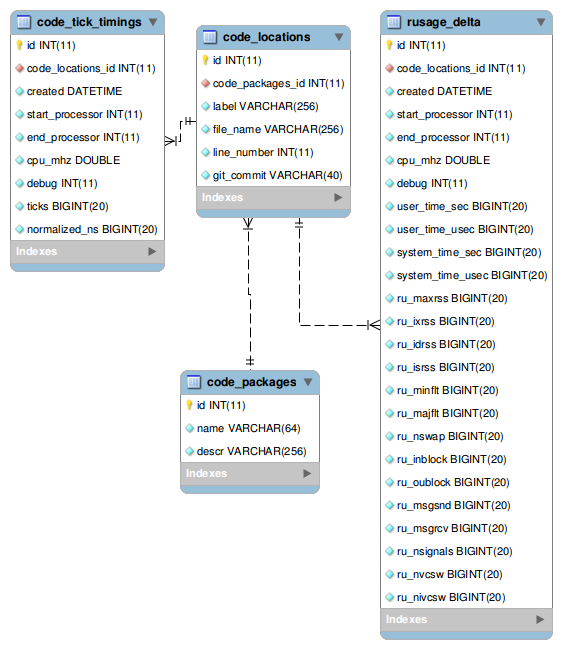
\includegraphics[width=.78\textwidth]{./images/code_metrics.png}   


   The details of the schema are not critical, but briefly, here is a
   description of the tables:


\begin{center}
\begin{tabular}{ll}
 Table                    &  Description                                                             \\
\hline
 code\_{}packages         &  A grouping mechanism. Code packages can be named                        \\
                          &  and described and then referenced for timing purposes.                  \\
 code\_{}locations        &  Describes specific locations in code that are to be timed.              \\
                          &  Includes \texttt{file\_name}, \texttt{line\_number} and references its  \\
                          &  \emph{code\_{}package}.                                                 \\
 code\_{}tick\_{}timings  &  Stores records of how long the block of code took.                      \\
 rusage\_{}delta          &  Stores records that include the change in \emph{resource utilization}   \\
                          &  used by the block of code. (This is linux specific)                     \\
\end{tabular}
\end{center}




   The following ruby script is used to generate the \emph{CRUD} support for this schema:


\lstset{language=Ruby}
\begin{lstlisting}
require 'codegen/database/database'
require 'odbc_ini'

DB = OdbcIni::ParsedEntries.instance.get_dsn_connection('code_metrics')
DB.loggers << Logger.new(STDOUT)
DB['DESCRIBE code_locations'].each do |row|
  puts row
end

database = 
  Codegen::Database.new({ 
                          :database_connection => DB,
                          :use_vector_on => [ :code_packages ],
                          :support_options => { 
                            :supports_delete_all => true, 
                            :supports_insert_ignore => [ :code_packages, :code_locations ],
                          },
                          :intrusive => true,
                        })
\end{lstlisting}



   One of the benefits of using a scripting language like ruby for
   code generation is you get the full power of the language and
   any/all supporting libraries. While the code above is clearly
   declarative, the bulk of the work is done in
   \texttt{codegen/database/database}, which makes use of the ruby \texttt{sequel}
   module to access the meta data defined by the schema. The benefit
   here is the approach can be used to generate supporting ORM code
   just by pointing a script at a database.

   A few samples pulled from the generated code to support the
   smallest table, \texttt{code\_packages} are shown below.

   Each database row is effectively a \texttt{pair}, specifically a \texttt{key} and
   \texttt{value}. This first class defines the value, which for a
   \texttt{code\_package} just aggregates the \texttt{name} and description (\texttt{descr})
   of the code package.

\pagebreak
\begin{itemize}

\item Table \texttt{Value} (i.e. the columns excluding the \emph{primary key})\\
\label{sec-4.2.1.1}



\lstset{language=C++}
\begin{lstlisting}

//! Encapsulates fields not in primary key of table <em>code_packages</em>
class Code_packages_value 
{
public:

  // Class enumerations
  enum Code_packages_value_fields {
    NAME_FIELD,
    DESCR_FIELD
  };

  // Number of entries in Code_packages_value_fields
  enum { CODE_PACKAGES_VALUE_FIELDS_NUMBER_ENTRIES = 2 };

  ...

  Code_packages_value(
    fcs::utils::Fixed_size_char_array< 64 > const& name,
    fcs::utils::Fixed_size_char_array< 256 > const& descr
  ) :
    name_(name),
    descr_(descr)
  {
  }

  Code_packages_value() :
    name_(fcs::utils::Fixed_size_char_array< 64 >()),
    descr_(fcs::utils::Fixed_size_char_array< 256 >()) 
  {
  }
  ...
  fcs::utils::Fixed_size_char_array< 64 > name_;
  fcs::utils::Fixed_size_char_array< 256 > descr_;
};
\end{lstlisting}



\pagebreak

\item Table \texttt{Key} (i.e. the \emph{primary key})\\
\label{sec-4.2.1.2}

  Similarly, the \texttt{key} is simply the primary id, wrapped in a class:


\lstset{language=C++}
\begin{lstlisting}
//! Encapsulates fields in primary key of table <em>code_locations</em>
class Code_locations_pkey 
{
public:

  explicit Code_locations_pkey(
    boost::int32_t id
  ) :
    id_(id)
  {
  }

  Code_locations_pkey() :
    id_(boost::int32_t()) 
  {
  }

  ...
  boost::int32_t id_;
};
\end{lstlisting}



\pagebreak
  So, these two classes define the structures that make up the records
  returned from the database when the full set of columns is
  queried. The next bit of code is what performs the \emph{CRUD}
  operations. This support file is quite large, especially considering
  the table this supports has only two non-primary fields (\texttt{name},
  \texttt{descr}).


\lstset{language=C++}
\begin{lstlisting}
//! Database object relational model support for table <em>code_locations</em>
template < typename PKEY_LIST_TYPE = std::list< Code_locations_pkey >,
           typename VALUE_LIST_TYPE = std::list< Code_locations_value >,
           typename LOCK_TYPE = boost::mutex,
           typename GUARD_TYPE = boost::lock_guard< LOCK_TYPE > > 
class Code_locations :
  public fcs::patterns::Singleton< Code_locations< PKEY_LIST_TYPE, VALUE_LIST_TYPE, LOCK_TYPE, GUARD_TYPE > > 
{
public:

  // Class typedefs
  typedef Code_locations_pkey Pkey_t;
  typedef Code_locations_value Value_t;
  typedef Code_locations_value_update Value_update_t;
  typedef PKEY_LIST_TYPE Pkey_list_t;
  typedef VALUE_LIST_TYPE Value_list_t;
  typedef LOCK_TYPE Lock_t;
  typedef GUARD_TYPE Guard_t;
  typedef std::pair< Code_locations_pkey, Code_locations_value > Row_t;
  typedef std::list< Row_t > Row_list_t;

protected:

  Code_locations() :
    connection_(Connection_code_metrics::get_instance()->get_connection()) 
  {
  }

public:

  inline void select_all_rows(Row_list_t &found, std::string const& where_clause = "")
    ...
  inline bool find_row(Code_locations_pkey const& desideratum, Code_locations_value & found)
    ...
  inline void find_rows(Pkey_list_t const& desideratum, Value_list_t & found)
    ...
  inline bool find_row_by_value(Row_t & desideratum)
    ...
  inline void insert(Row_t const& nascent)
    ...
  inline void insert_ignore(Row_t const& nascent)
    ...
  inline void insert(Row_list_t const& nascent, int stream_buffer_size = 1)
    ...
  inline void update(Row_list_t const& changing)
    ...
  inline void update(Code_locations_pkey const& changing, 
                     Code_locations_value_update const& updates)
    ...

  inline void delete_rows(Pkey_list_t const& moribund, size_t max_per_call = 0)
    ...

  inline size_t delete_all_rows()
    ...
private:
  otl_connect * connection_;
  friend class fcs::patterns::Singleton_impl< Code_locations >;
};
\end{lstlisting}



\pagebreak

\item Sample Usage\\
\label{sec-4.2.1.3}


     The following demonstrates a simple \emph{C} from the \emph{CRUD} by making
     use of the \texttt{insert\_ignore} function. This function inserts the
     code package (ignoring any error if already present).


\lstset{language=C++}
\begin{lstlisting}
Code_packages<>::Row_t code_packages;
code_packages.second.name_ = api_name;
code_packages.second.descr_ = api_description;
Code_packages<>::Pointer_t code_packages_table(Code_packages<>::get_instance());
code_packages_table->insert_ignore(code_packages);
\end{lstlisting}



\end{itemize} % ends low level
\subsubsection{ORM Select Example}
\label{sec-4.2.2}

    
    Similar to the \emph{CRUD} operations, table selects can also be
    generated.

    The following ruby select definition can drive generation of the
    code supporting the query. To generate the code the process must
    understand the types of the columns and have proper mappings to
    corresponding \texttt{C++} types. Much of this can be retrieved from the
    database meta-data.


\lstset{language=Ruby}
\begin{lstlisting}
"
select 
  CP.name as package_name,
  CL.label,
  CL.file_name,
  RD.created,
  CL.line_number,
  CL.git_commit,
  RD.!/id|created$/
from 
  code_locations as CL, 
  code_packages as CP,
  rusage_delta as RD
where  
  CL.label like {presubstitute(:cpp_type => 'std::string', :name => 'label')} and
  CP.name like {substitute('CP.name', :package_name)} and
  RD.code_locations_id = CL.id and
  CL.code_packages_id = CP.id
order by
  CP.name,
  CL.label,
  RD.created
}
"
\end{lstlisting}



\pagebreak
    The corresponding code generates a basic class for the returned columns:

\lstset{language=C++}
\begin{lstlisting}
  struct Rusage_delta_by_package_label 
  {

    Rusage_delta_by_package_label() :
      package_name_(fcs::utils::Fixed_size_char_array< 64 >()),
      label_(fcs::utils::Fixed_size_char_array< 256 >()),
      file_name_(fcs::utils::Fixed_size_char_array< 256 >()),
      created_(otl_datetime()),
      line_number_(boost::int32_t()),
      git_commit_(fcs::utils::Fixed_size_char_array< 40 >()),
      start_processor_(boost::int32_t()),
      end_processor_(boost::int32_t()),
      cpu_mhz_(double()),
      debug_(boost::int32_t()),
      user_time_sec_(otl_bigint()),
      user_time_usec_(otl_bigint()),
      system_time_sec_(otl_bigint()),
      system_time_usec_(otl_bigint()),
      ru_maxrss_(otl_bigint()),
      ...
    {
    }
    ...
};
\end{lstlisting}


  
\pagebreak
    As well as a class to perform the query:


\lstset{language=C++}
\begin{lstlisting}
class Rusage_delta_by_package_label_query 
{
public:

  // Class typedefs
  typedef std::list< Rusage_delta_by_package_label > Row_list_t;

  Rusage_delta_by_package_label_query(
    fcs::utils::Fixed_size_char_array< 64 > const& package_name,
    std::string const& label
  ) :
    query_result_(),
    query_("select\n"
    "  CP.name as package_name,\n"
    "  CL.label as label,\n"
    "  CL.file_name as file_name,\n"
    "  RD.created as created,\n"
    "  CL.line_number as line_number,\n"
    ...
    "from\n"
    "  code_locations as CL, \n"
    "  code_packages as CP,\n"
    "  rusage_delta as RD\n"
    "where\n"
    "  CL.label like %1% and\n"
    "  CP.name like :package_name<char[64]> and\n"
    "  RD.code_locations_id = CL.id and\n"
    "  CL.code_packages_id = CP.id\n"
    "order by\n"
    "  CP.name,\n"
    "  CL.label,\n"
    "  RD.created"),
    package_name_(package_name),
    label_(label)
  {
    ctor_member_init();
  }

  void ctor_member_init() {
    using boost::format;
    using boost::io::group;
    std::ostringstream query_text;
    query_text << format(query_.c_str()) % fcs::orm::sql_quote(label_);
    otl_stream stream(
      50, query_text.str().c_str(),
      *Connection_code_metrics::get_instance()->get_connection());
    stream 
      << package_name_
    ;
    while(!stream.eof()) {
      Rusage_delta_by_package_label rusage_delta_by_package_label;
      stream
        >> rusage_delta_by_package_label.package_name_
        >> rusage_delta_by_package_label.label_
        >> rusage_delta_by_package_label.file_name_
        >> rusage_delta_by_package_label.created_
        >> rusage_delta_by_package_label.line_number_
        ...
      query_result_.push_back(rusage_delta_by_package_label);
    }
  }
\end{lstlisting}


    
\pagebreak

    And a snippit of code showing the usage:


\lstset{language=C++}
\begin{lstlisting}
Rusage_delta_by_package_label_query 
  query(options.package_.c_str(), options.location_label_);
query.print_query_results_as_table(std::cout);
\end{lstlisting}



\section{Templates}
\label{sec-5}


  Support for the code generation is driven by ruby referencing a set
  of hand-written \emph{Tenjin} templates. In this example class
  \texttt{Change\_tracker}, the member accessors (actually all code outside of
  the \emph{Protect Blocks}) are auto-generated.


\lstset{language=C++}
\begin{lstlisting}
  template < typename T > 
  class Change_tracker 
  {
  public:

    /////////////////////////////////////////////////////////////////
    // member accessors
    /////////////////////////////////////////////////////////////////
    T current() const {
      return current_;
    }

    T previous() const {
      return previous_;
    }

  
// custom <Change_tracker public header section>

    Change_tracker(T current) : current_(current), previous_(T()) {
    }

    void next_value(T next_value) {
      previous_ = current_;
      current_ = next_value;
    }

// end <Change_tracker public header section>

  private:
    T current_;
    T previous_;
  };
\end{lstlisting}



\pagebreak
  The member accessors themselves are generated from the following
  template. In this case the two members are \emph{Read Only}, so only
  getters are supplied. The potential accessors are generated
  consistently based on this breakdown of desired functionality:
\begin{itemize}
\item \emph{Read Only} : A read accessor is generated
\item \emph{Read Write} : Both read and write accessors are generated
\item \emph{Inaccessible} : Neither accessor is generated, this is the
    default.
\end{itemize}
  Because this is \texttt{C++} which allows for implementation to be separated
  from interface, the option exists to have the accessors be simply
  declared, thus hiding the implementation in a \emph{cpp} file. The
  default is to just inline the accessors.


\lstset{language=Ruby}
\begin{lstlisting}
<?rb i=Codegen.single_indent() ?>
<?rb if not @cls.readable_members.empty? or not @cls.writable_members.empty? ?>
#{i}/////////////////////////////////////////////////////////////////
#{i}// member accessors
#{i}/////////////////////////////////////////////////////////////////
<?rb end ?>
<?rb @cls.members.each do |m| ?>
<?rb start_capture :member_accessors ?>
    <?rb if @cls.readable_members.include? m ?>
        <?rb if m.brief and @cls.accessor_docs ?>
//! reader for #{m.name} <B>#{m.brief}</B>
        <?rb end ?>
        <?rb if m.hide_impl ?>
#{m.reader_decl}
        <?rb else ?>        
#{m.reader_impl}
        <?rb end ?>
    <?rb end ?>
    <?rb if @cls.writable_members.include? m ?>
            <?rb if m.brief and @cls.accessor_docs ?>
//! writer for #{m.name} <B>#{m.brief}</B>
            <?rb end ?>
        <?rb if m.hide_impl ?>
#{m.writer_decl}
        <?rb else ?>        
#{m.writer_impl}
        <?rb end ?>
        <?rb if m.pass_by_ref ?>
            <?rb if m.brief and @cls.accessor_docs ?>
//! non-const reader for #{m.name} <B>#{m.brief}</B>
            <?rb end ?>
          <?rb if m.hide_impl ?>
#{m.reader_decl_non_const}
          <?rb else ?>        
#{m.reader_impl_non_const}
          <?rb end ?>
        <?rb end ?>
    <?rb end ?>
<?rb stop_capture ?>
<?rb   if @member_accessors and (@member_accessors.length > 0) ?>
#{m.ifdef(Codegen.indent_text(@member_accessors, 0))}

<?rb   end ?>
<?rb end ?>
\end{lstlisting}




  Another feature of members and their accessors is the ability to
  conditionally include them. For instance, maybe in a \texttt{DEBUG} mode
  you would like to track the \texttt{hit\_count} of a certain event. By
  specifying \texttt{ifdef\_identifier} in the member definition, this can be
  achieved.

  So, for example, the additional member \texttt{hit\_count} here:


\lstset{language=Ruby}
\begin{lstlisting}
:members => [
             { 
               :cpp_type => 'T',
               :name => 'current',
               :access => :read_only,
             },
             { 
               :cpp_type => 'T',
               :name => 'previous',
               :access => :read_only,
             },
             { 
               :cpp_type => 'int',
               :name => 'hit_count',
               :ifdef_identifier => 'DEBUG',
               :access => :read_only,
             },
            ],
\end{lstlisting}



   will cause updates like:


\lstset{language=C++}
\begin{lstlisting}
  template < typename T > 
  class Change_tracker 
  {
  public:

    /////////////////////////////////////////////////////////////////
    // member accessors
    /////////////////////////////////////////////////////////////////
    T current() const {
      return current_;
    }

    T previous() const {
      return previous_;
    }

#if defined(DEBUG)
    int hit_count() const {
      return hit_count_;
    }
#endif

  
// custom <Change_tracker public header section>

    Change_tracker(T current) : current_(current), previous_(T()) {
    }

    void next_value(T next_value) {
      previous_ = current_;
      current_ = next_value;
    }

// end <Change_tracker public header section>

  private:
    T current_;
    T previous_;
#if defined(DEBUG)
    int hit_count_;
#endif
  };
\end{lstlisting}




\subsection{Customizing in \textbf{Ruby} vs \textbf{Templates}}
\label{sec-5.1}


   Not all code text needs to be created from a template. Sometimes it
   is more convenient to just build up snippets of text from ruby
   code, rather than dedicate a template for the purpose.  For
   example, a common need in \texttt{C++} may be to store a class in a set or
   as the key to a map. This requires the class designer to write an
   \texttt{operator<} method, which can be quite tedious as the fields of the
   class grow. Including this method in a generated C++ file just
   requires the addition of \texttt{:comparable => true} to the class
   specification. In fact, part of the elided code in the
   \texttt{Code\_packages\_value} class is such a function, since it is often
   desirable to be able to store records returned from the database in
   a \emph{std::set} or \emph{std::map}.


\lstset{language=C++}
\begin{lstlisting}
bool operator<(Code_packages_value const& rhs) const {
    return
        ((name_ != rhs.name_)? name_ < rhs.name_ : (
        ((descr_ != rhs.descr_)? descr_ < rhs.descr_ : (false
        ))));
}
\end{lstlisting}



   As the number of fields grows, so does the complexity:

\lstset{language=C++}
\begin{lstlisting}
bool operator<(Code_locations_value const& rhs) const {
    return
        ((code_packages_id_ != rhs.code_packages_id_)? code_packages_id_ < rhs.code_packages_id_ : (
        ((label_ != rhs.label_)? label_ < rhs.label_ : (
        ((file_name_ != rhs.file_name_)? file_name_ < rhs.file_name_ : (
        ((line_number_ != rhs.line_number_)? line_number_ < rhs.line_number_ : (
        ((git_commit_ != rhs.git_commit_)? git_commit_ < rhs.git_commit_ : (false
        ))))))))));
}
\end{lstlisting}



\section{C++ Features}
\label{sec-6}

\subsection{Consistent Libraries}
\label{sec-6.1}

   
   As progress has been made in the \texttt{C++} development community, it
   seems there has been a shift away from \texttt{C++} libraries (i.e. \texttt{.lib}
   on windows and \texttt{.a} on linux files) and towards header only
   libraries. At the time this support was originally developed, my
   focus was code generation to allow for separation of interface and
   implementation (as described in \emph{Large Scale C++ Software Design}
   Lakos), so libraries were critical. Many of the messy issues with
   Windows development were handled, like support for exposing symbols
   in a dll (i.e. \texttt{\_\_declspec(dllexport)} defines) and exporting
   classes. As time went on the focus was much more geared toward
   linux. So, beware that some of the windows support may now be
   suspect and require a revamp.

   
   For an included example of a library, see
   \texttt{lib\_gui\_environment.rb}. For an included example of header only
   library, see \texttt{lib\_utils.rb} or \texttt{lib\_patterns.rb}.


\subsection{Consistent Apps}
\label{sec-6.2}


   A typical application definition looks like this the
   following. 


\lstset{language=Ruby}
\begin{lstlisting}
app = Application.new(
                      { 
                        :name => 'cpu_info',
                        :log_pantheios_fe => true,
                        :program_options => program_options,
                        :classes => [],
                        :folder => 'cpu_info',
                        :namespace => [ 'fcs', 'linux_specific', ],
                        :app_includes => 
                        [ 
                         'fcs/linux_specific/cpu_info.hpp',
                        ],
                        :jam_requirements => [ 
                                              '$(PANTHEIOS_LIBS)',
                                              '/site-config//boost_program_options',
                                              '/site-config//boost_regex',
                                             ],
                      }
                      )
\end{lstlisting}




   This defines an application called \emph{cpu\_{}info} which just dumps the
   parsed data from the linux \texttt{cpuinfo} file. The specification
   provides:
\begin{itemize}
\item \texttt{:name}: Name of the app. By default, all apps are placed in
     \texttt{cpp/apps/} in a folder corresponding to this name
\item \texttt{:log\_panntheios\_fe}: Whether to incluce pantheios logging front
     end
\item \texttt{:program\_options} Defined higher up in the ruby file, this data
     describes the command line options of the app.
\item \texttt{:classes} The list of top-level classes. In this case, no
     classes are required as the work is done in the included
     libraries.
\item \texttt{:folder} Optionally specifies the folder under \texttt{cpp/apps/} to
     place this app. The purpose is to group related apps together.
\item \texttt{:app\_includes} Specifies the files to include for this top-level
     file(s).
\item \texttt{:jam\_requirements} Specifies the library requirements for this
     app.
\end{itemize}
\subsubsection{Consistent Logging}
\label{sec-6.2.1}


    The logging package used in this setup is \emph{Pantheios}
    (\href{http://www.pantheios.org/}{http://www.pantheios.org/}). When an app definition specifies
    \texttt{:log\_panntheios\_fe}, the following code is included in the app
    cpp file. This sets the \texttt{processIdentity}, so the log messages are
    labeled, as well as provides a \texttt{set\_log\_level} setting to the app.


\lstset{language=C++}
\begin{lstlisting}
////////////////////////////////////////////////////////////////////////////////
// The following pantheios related functions provide basic selective
// logging support
////////////////////////////////////////////////////////////////////////////////
PANTHEIOS_CALL(int) pantheios_fe_init(void*, void** ptoken) { 
  *ptoken = NULL; 
  return 0; 
}

PANTHEIOS_CALL(void) pantheios_fe_uninit(void*) {}

PANTHEIOS_CALL(PAN_CHAR_T const*) pantheios_fe_getProcessIdentity(void*)
{
  return ("cpu_info");
}

::pantheios::pan_sev_t app_log_severity_s(::pantheios::SEV_ERROR);

namespace fcs { 
namespace utils {

namespace {
  boost::mutex protect_severity_s;
}

  void set_log_level(::pantheios::pan_sev_t new_severity) {
    boost::mutex::scoped_lock lock(protect_severity_s);
    app_log_severity_s = new_severity;
  }
}
}

PANTHEIOS_CALL(int) pantheios_fe_isSeverityLogged(void*, int severity, int)
{
  return severity <= app_log_severity_s;
}
\end{lstlisting}



  The \emph{program options} support, described below, allows for the
  consistent controlling the log level from the command line, via the
  \texttt{:standard\_logging} setting.

\subsubsection{Consistent Program Options}
\label{sec-6.2.2}


  Setting up program options for an application can be a pain. The
  \texttt{CppOptionParserGenerator} allows consistent definition of program
  options. All program command line option support is fully generated
  based on these options specifications. A sample, below shows the
  simplest of command options sets for an app called \texttt{display\_csv},
  which displays a csv file in a Qt table view. This app takes one
  command line option, (\texttt{-c} to specify the path of the csv file to
  display)


\lstset{language=Ruby}
\begin{lstlisting}
program_options = 
  CppOptionParserGenerator.new( {
                                  :name => 'Display_csv',
                                  :standard_logging => true,
                                  :brief => 'Wraps a model on a csv for display in Qt',
                                  :descr => " 
Takes one or more csv files and for each wraps a view on it.
",
                                  :options => [
                                               { 
                                                 :name => 'csv_file',
                                                 :short_name => 'c',
                                                 :cpp_type => 'std::string',
                                                 :descr => 'Csv file path(s) to open',
                                                 :is_multiple => true,
                                               },
                                              ],

                                })
\end{lstlisting}



  The inclusion of this definition causes the generation of
  \texttt{display\_csv\_program\_options.[ch]pp} files.

  In addition it generates the code to read and parse the command line
  options:


\lstset{language=C++}
\begin{lstlisting}
int main(int argc, char** argv, char** envp) {

  // Get the user supplied program options
  using namespace fcs::app;
  Display_csv_program_options options;
  try {
    read_parameters(options, argc, argv);
    if(options.help_) {
      std::cout << get_display_csv_options_description();
      std::cout.flush();
      return 0;
    }
  } catch(std::exception const& excp) {
    std::cout << "Caught exception:" << excp.what() << std::endl;
    return -1;
  }

  if(options.parsed_program_options_.count("log_level")) {
    fcs::utils::set_log_level(options.log_level_);
  }

  pantheios::log(PANTHEIOS_SEV_DEBUG, "app display_csv run with main(", 
    pantheios::args(argc, argv, pantheios::args::arg0FileOnly), ")");
  
// custom <main_body>
...
// end <main_body> 
  return 0;
}
\end{lstlisting}



  Now when this app is run, the following options are available.


\lstset{language=Ruby}
\begin{lstlisting}
Wraps a model on a csv for display in Qt

 
Takes one or more csv files and for each wraps a view on it.


Allowed Options:
  -h [ --help ]         Prints this help message
  -c [ --csv_file ] arg Csv file path(s) to open <std::string>
  --log_level arg (=3)  Number in (EMERGENCY=0, ALERT=1, CRITICAL=2, ERROR=3, 
                        WARNING=4, NOTICE=5, INFO=6, DEBUG=7) <int>
\end{lstlisting}



  Note that \texttt{--log\_level} option was included because of the
  \texttt{:standard\_logging} setting of the program options. A similar option
  \texttt{:standard\_otl\_logging} can be specified to allow for logging of
  database commands sent to the server. For example, app
  \texttt{timing\_report} just queries the database for timing information on
  blocks of code. The following definition includes
  \texttt{:standard\_otl\_logging}.


\lstset{language=Ruby}
\begin{lstlisting}
program_options = 
  CppOptionParserGenerator.new( {
                                  :name => 'Timing_report',
                                  :standard_logging => true,
                                  :standard_otl_logging => true,
                                  :brief => 'Reports on rusage or clock timings',
                                  :descr => " 
Given package, location, or other filters will report on timings
",
                                  :options => [
                                               { 
                                                 :name => 'package',
                                                 :short_name => 'p',
                                                 :cpp_type => 'std::string',
                                                 :descr => 'Package to report on',
                                                 :default_value => '"%"',
                                               },
                                               { 
                                                 :name => 'location_label',
                                                 :short_name => 'l',
                                                 :cpp_type => 'std::string',
                                                 :descr => 'Label to report on',
                                                 :default_value => '"%"',
                                               },
                                               { 
                                                 :name => 'rusage',
                                                 :short_name => 'r',
                                                 :cpp_type => 'bool',
                                                 :descr => 'If true reports rusage',
                                                 :default_value => false,
                                               },
                                               { 
                                                 :name => 'ticks',
                                                 :short_name => 't',
                                                 :cpp_type => 'bool',
                                                 :descr => 'If true reports clock ticks',
                                                 :default_value => false,
                                               },
                                              ],

                                })
\end{lstlisting}



   The inclusion of the \texttt{:standard\_otl\_logging} is what causes the
   addition of the \texttt{--otl\_log\_level} arg below.


\lstset{language=Ruby}
\begin{lstlisting}

Reports on rusage or clock timings

 
Given package, location, or other filters will report on timings


Allowed Options:
  -h [ --help ]                    Prints this help message
  -p [ --package ] arg (=%)        Package to report on <std::string>
  -l [ --location_label ] arg (=%) Label to report on <std::string>
  -r [ --rusage ]                  If true reports rusage
  -t [ --ticks ]                   If true reports clock ticks
  --log_level arg (=3)             Number in (EMERGENCY=0, ALERT=1, CRITICAL=2,
                                   ERROR=3, WARNING=4, NOTICE=5, INFO=6, 
                                   DEBUG=7) <int>
  --otl_log_level arg              Number in mask {Level_1=1 
                                   (connect/disconnect), Level_2=2, Level_3=4 
                                   (selects), Level_4=8 (selects + parms), 
                                   Level_5=16 (parm streaming)} <int>
\end{lstlisting}



   Now, when run as \texttt{timing\_report.cpp --otl\_log\_level=4}, the SQL
   selects are logged:


\begin{lstlisting}
OTL => otl_stream(this=0x7fff0c6c6c10)::open(buffer_size=50, sqlstm=select
  CP.name as package_name,
  CL.label as label,
  CL.file_name as file_name,
  RD.created as created,
  CL.line_number as line_number,
  CL.git_commit as git_commit,
  RD.start_processor as start_processor,
  RD.end_processor as end_processor,
  RD.cpu_mhz as cpu_mhz,
  RD.debug as debug,
  RD.user_time_sec as user_time_sec,
  RD.user_time_usec as user_time_usec,
  RD.system_time_sec as system_time_sec,
  RD.system_time_usec as system_time_usec,
  RD.ru_maxrss as ru_maxrss,
  ...
from
  code_locations as CL, 
  code_packages as CP,
  rusage_delta as RD
where
  CL.label like "%" and
  CP.name like :package_name<char[64]> and
  RD.code_locations_id = CL.id and
  CL.code_packages_id = CP.id
order by
  CP.name,
  CL.label,
  RD.created, connect=0x245a5a0, implicit_select=0);
OTL => otl_stream(this=0x7fff0c6c6c10)::close();
OTL => otl_stream(this=0x7fff0c6c6d70)::open(buffer_size=50, sqlstm=select
  CP.name as package_name,
  CL.label as label,
  CL.file_name as file_name,
  CTT.created as created,
  CL.line_number as line_number,
  CL.git_commit as git_commit,
  CTT.start_processor as start_processor,
  CTT.end_processor as end_processor,
  CTT.cpu_mhz as cpu_mhz,
  CTT.debug as debug,
  CTT.ticks as ticks,
  CTT.normalized_ns as normalized_ns
from
  code_locations as CL, 
  code_packages as CP,
  code_tick_timings as CTT
where
  CL.label like :label<char[256]> and
  CP.name like :package_name<char[64]> and
  CTT.code_locations_id = CL.id and
  CL.code_packages_id = CP.id
order by
  CP.name,
  CL.label,
  CTT.created, connect=0x245a5a0, implicit_select=0);
OTL => otl_stream(this=0x7fff0c6c6d70)::close();
|---------------|---------...|--------------...|--------------------|-----...|------------...
| package_name_ | label_  ...| file_name_   ...| created_           | line...| git_commit_
|---------------|---------...|--------------...|--------------------|-----...|------------...
| fcs::orm::orm | Rusage T...| test_block_tr...| 1/14/2013 16:52:7  | 60  ...| 8d3771cb9cb...
| fcs::orm::orm | Rusage T...| test_block_tr...| 1/14/2013 17:11:20 | 61  ...| 8d3771cb9cb...
| fcs::orm::orm | Rusage T...| test_block_tr...| 1/14/2013 17:13:39 | 61  ...| 8d3771cb9cb...
| fcs::orm::orm | Rusage T...| test_block_tr...| 1/14/2013 16:52:3  | 60  ...| 8d3771cb9cb...
| fcs::orm::orm | Rusage T...| test_block_tr...| 1/14/2013 17:11:16 | 61  ...| 8d3771cb9cb...
\end{lstlisting}




\subsubsection{Consistent Signal Handling}
\label{sec-6.2.3}

    
    When defining an app, by default signal handling is provided. To
    not include signal handling, turn the \texttt{:app\_sig\_handler} flag
    off. For example, consider the definition of \texttt{cpu\_info}.  Since
    there is no disabling of \texttt{:app\_sig\_handler}, the following sig
    handler code is included in the app. This handler just intercepts
    signals in \emph{Release} and provides an \texttt{add\_handler} method to plug
    in a user defined handler.


\lstset{language=C++}
\begin{lstlisting}
#if !defined(DEBUG)
fcs::app_sig_handler::Application_signal_handler<>::Pointer_t
app_sig_handler_s(fcs::app_sig_handler::Application_signal_handler<>::get_instance());
#endif

int main(int argc, char** argv, char** envp) {
...
}
\end{lstlisting}


    
\subsection{Consistent Testing}
\label{sec-6.3}


   The file structure of generated code is the same as that of the
   boost projects. So the top level is \texttt{fcs} as opposed to \texttt{boost}.


\begin{center}
\begin{tabular}{ll}
 Location                                               &  Description                                   \\
\hline
 cpp                                                    &  Root for a cpp files                          \\
 cpp/fcs                                                &  Top level \emph{package} for support files    \\
 cpp/fcs/utils/synch                                    &  Example of headers for header only ``lib''    \\
                                                        &  fcs::utils::synch which has traits types for  \\
                                                        &  boost locking and tbb locking                 \\
 cpp/libs                                               &  Top level for libs and optionally unit tests  \\
 cpp/libs/fcs/utils/unit\_{}test/test\_{}streamers.cpp  &  Example of unit\_{}test for streamers.        \\
\end{tabular}
\end{center}




   To generate code to support the testing of a class include the
   \texttt{:include\_unit\_test} option. For example, in \texttt{lib\_patterns.rb} the
   \texttt{Signaller} class specification has \texttt{:include\_unit\_test =>    true}. By doing this the file
   \texttt{cpp/libs/fcs/patterns/unit\_test/test\_signaller.cpp} is created as
   well as a \texttt{Jamfile} to run the test. Then it is the developers job
   to fill in the test code.

\section{Code Generation/C++ Requirements}
\label{sec-7}


\subsection{Ruby Requirements}
\label{sec-7.1}

\begin{itemize}
\item \textbf{tenjin}: Template engine
\item \textbf{grit}: Used to access \emph{git} to get the current commit so \texttt{C++}
    binaries can be tracked to a \emph{git} commit
\item \textbf{mysql}: For accessing MySQL specifically (the focus of this ORM)
\item \textbf{sequel} For accessing a database
\item \textbf{terminal-table}: For printing ASCII like tables from \textbf{ruby}
\item \textbf{parseconfig}: For parsing config files (used to parse \texttt{\textasciitilde{}/.odbc\_ini})
\end{itemize}
  
\subsection{C++ Requirements}
\label{sec-7.2}


\begin{itemize}
\item \textbf{boost}: Used throughout
\item \textbf{stlsoft}: Prereq for \textbf{pantheios}
\item \textbf{fastformat}: Prereq for \textbf{pantheios}
\item \textbf{pantheios}: \href{http://www.pantheios.org/}{http://www.pantheios.org/} A fast general purpose
    logging framework.
\item \textbf{otl}: \href{http://otl.sourceforge.net}{http://otl.sourceforge.net} Template library Used for
    accessing relational databases using ODBC
\item \textbf{boost-build}: Build scripts are generated as \texttt{Jamfiles}. In the
    future this should probably be upgraded to \texttt{CMake} since the \emph{long     term} future of \textbf{boost-build} is in question.
\end{itemize}
\section{D Features}
\label{sec-8}

  TBD\ldots{}

\end{document}
